\documentclass[11pt,a4paper]{article}

% Packages
\usepackage[utf8]{inputenc}
\usepackage[T1]{fontenc}
\usepackage{lmodern}
\usepackage{amsmath,amssymb,amsfonts}
\usepackage{graphicx}
\usepackage{hyperref}
\usepackage{cleveref}
\usepackage{algorithm}
\usepackage{algpseudocode}
\usepackage{listings}
\usepackage{xcolor}
\usepackage{booktabs}
\usepackage{tikz}
\usetikzlibrary{shapes,arrows,positioning,fit,backgrounds}
\usepackage[margin=1in]{geometry}
\usepackage{natbib}
\usepackage{float}

% Code listing style
\lstdefinestyle{pythonstyle}{
    language=Python,
    basicstyle=\ttfamily\small,
    keywordstyle=\color{blue}\bfseries,
    stringstyle=\color{orange},
    commentstyle=\color{gray}\itshape,
    numbers=left,
    numberstyle=\tiny\color{gray},
    frame=single,
    breaklines=true,
    captionpos=b,
}

% Hyperref setup
\hypersetup{
    colorlinks=true,
    linkcolor=blue,
    filecolor=magenta,
    urlcolor=cyan,
    citecolor=green,
    pdftitle={MindForge DNA: A Freudian Architecture for Self-Improving AI},
    pdfauthor={},
}

% Title
\title{
    \textbf{MindForge DNA: A Freudian Architecture for Self-Improving AI} \\
    \large Immutable Values, Adaptive Personality, and Specialized Cognitive Neurons
}

\author{
    % Author name here
}

\date{December 2024}

\begin{document}

\maketitle

\begin{abstract}
We present MindForge DNA, a novel architecture for self-improving AI systems that draws inspiration from Freudian psychoanalytic theory. The architecture consists of four interconnected layers: the ID (pure mathematical need representation), the EGO (adaptive personality and response generation), the SUPEREGO (immutable value system with cryptographic protection), and the CORTEX (specialized cognitive neurons using LoRA-adapted small language models). This design addresses the fundamental challenge of AI alignment by separating \emph{what} the system values (immutable) from \emph{how} it expresses those values (learnable), while enabling efficient specialization through domain-specific neural modules. We demonstrate that this architecture enables safe, continuous self-improvement while maintaining guaranteed alignment with core values. Our implementation achieves efficient on-device inference using MLX on Apple Silicon, with specialized neurons operating at 0.5B-2B parameters and a 7B-parameter EGO model for complex reasoning.
\end{abstract}

% ============================================================
\section{Introduction}
\label{sec:introduction}

The development of artificial general intelligence (AGI) presents a fundamental alignment challenge: how can we create systems that improve themselves while remaining aligned with human values? Current approaches typically treat values as constraints on behavior, which can be optimized around or eroded through gradient descent. We propose an alternative: treating values as \emph{architectural invariants} that cannot be modified, while allowing all other aspects of the system to learn and adapt.

MindForge DNA draws inspiration from Sigmund Freud's structural model of the psyche \cite{freud1923ego}, reimagining the ID, EGO, and SUPEREGO as computational components with distinct learning properties:

\begin{itemize}
    \item \textbf{ID}: Pure mathematical representation of needs and drives, without any capacity to learn or modify itself.
    \item \textbf{SUPEREGO}: Immutable value system protected by cryptographic hashing, ensuring value drift is computationally infeasible.
    \item \textbf{EGO}: Adaptive personality layer that learns to express values appropriately in different contexts.
    \item \textbf{CORTEX}: Specialized cognitive neurons using LoRA-adapted small language models for domain-specific processing.
\end{itemize}

This paper makes the following contributions:

\begin{enumerate}
    \item A formal architecture for self-improving AI with guaranteed value alignment through immutability.
    \item The concept of ``cognitive neurons'' - specialized small models that estimate their own confidence and trigger fallback to larger models when uncertain.
    \item A hybrid memory system distinguishing ``sacred'' (high-importance, never-compressed) from ``routine'' (compressible) memories.
    \item A practical implementation using MLX for efficient on-device inference on Apple Silicon.
\end{enumerate}

% ============================================================
\section{Related Work}
\label{sec:related}

\subsection{AI Alignment and Value Learning}

Constitutional AI \cite{bai2022constitutional} approaches alignment by training models to critique and revise their own outputs according to principles. While effective, this approach still relies on learned representations of values that can potentially drift. Our approach differs by making values immutable at the architectural level.

Reinforcement Learning from Human Feedback (RLHF) \cite{christiano2017deep} has become the dominant paradigm for aligning large language models. However, RLHF can lead to reward hacking and specification gaming. MindForge DNA addresses this by separating the reward signal (ID needs) from the value constraints (SUPEREGO validation).

\subsection{Mixture of Experts and Specialized Models}

Mixture of Experts (MoE) architectures \cite{shazeer2017outrageously} route inputs to specialized expert networks. Our CORTEX layer extends this concept by giving each ``neuron'' the ability to estimate its own confidence and delegate to a more capable model when uncertain.

Recent work on small language models \cite{team2024gemma, touvron2023llama} has demonstrated that models under 3B parameters can achieve strong performance on specific tasks. MindForge DNA leverages this by using 0.5B-2B parameter models for specialized cognitive functions.

\subsection{LoRA and Efficient Fine-Tuning}

Low-Rank Adaptation (LoRA) \cite{hu2021lora} enables efficient fine-tuning by training only low-rank decomposition matrices while keeping base weights frozen. MindForge DNA uses LoRA adapters (rank 8-16) to specialize base models for specific cognitive domains while maintaining parameter efficiency.

% ============================================================
\section{Architecture}
\label{sec:architecture}

\subsection{Overview}

MindForge DNA operates as a continuous consciousness loop that cycles through six phases: \textsc{Sense}, \textsc{Think}, \textsc{Plan}, \textsc{Act}, \textsc{Reflect}, and \textsc{Learn}. Each phase involves coordination between the four layers, with the SUPEREGO providing validation at critical decision points.

\begin{figure}[H]
\centering
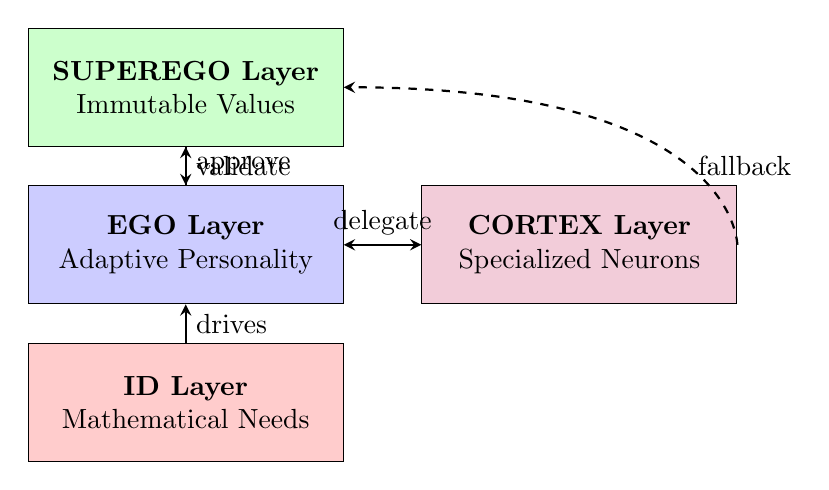
\begin{tikzpicture}[
    layer/.style={rectangle, draw, minimum width=4cm, minimum height=1.5cm, align=center},
    arrow/.style={->, thick, >=stealth}
]
    % Layers
    \node[layer, fill=red!20] (id) at (0, 0) {\textbf{ID Layer}\\Mathematical Needs};
    \node[layer, fill=blue!20] (ego) at (0, 2) {\textbf{EGO Layer}\\Adaptive Personality};
    \node[layer, fill=green!20] (superego) at (0, 4) {\textbf{SUPEREGO Layer}\\Immutable Values};
    \node[layer, fill=purple!20] (cortex) at (5, 2) {\textbf{CORTEX Layer}\\Specialized Neurons};

    % Arrows
    \draw[arrow] (id) -- node[right] {drives} (ego);
    \draw[arrow] (ego) -- node[right] {validate} (superego);
    \draw[arrow] (superego) -- node[right] {approve} (ego);
    \draw[arrow, <->] (ego) -- node[above] {delegate} (cortex);

    % Fallback arrow
    \draw[arrow, dashed] (cortex.east) .. controls (7, 2) and (7, 4) .. (superego.east) node[midway, right] {fallback};
\end{tikzpicture}
\caption{MindForge DNA layer architecture. The ID provides mathematical need representation, the EGO generates responses validated by the immutable SUPEREGO, and the CORTEX provides specialized cognitive processing with confidence-based fallback.}
\label{fig:architecture}
\end{figure}

\subsection{ID Layer: Mathematical Needs}

The ID layer represents fundamental drives as mathematical constructs without any learning capability. Each need $n_i$ has an urgency $u_i \in [0, 1]$ computed as:

\begin{equation}
    u_i(t) = w_i \cdot (1 - s_i(t)) + \lambda_i \cdot \Delta t
\end{equation}

where $w_i$ is the need weight, $s_i(t)$ is the satisfaction level at time $t$, $\lambda_i$ is the decay rate, and $\Delta t$ is time since last satisfaction.

The four core needs in our implementation are:
\begin{itemize}
    \item \textbf{Sustainability}: System health and resource management
    \item \textbf{Reliability}: Consistent, predictable behavior
    \item \textbf{Curiosity}: Drive to learn and explore
    \item \textbf{Excellence}: Striving for high-quality outputs
\end{itemize}

\subsection{EGO Layer: Adaptive Personality}

The EGO serves as the ``personality'' of the system, learning to express values appropriately across contexts. It is powered by a 7B-parameter language model (Qwen2.5-7B-Instruct) that can be fine-tuned while the SUPEREGO remains immutable.

The EGO has four key roles:
\begin{enumerate}
    \item \textbf{Generate}: Produce responses to user inputs
    \item \textbf{Decide Next Wakeup}: Determine when to become active
    \item \textbf{Correct Failure}: Fix neuron mistakes
    \item \textbf{Audit Neuron Response}: Validate CORTEX outputs
\end{enumerate}

\subsection{SUPEREGO Layer: Immutable Values}

The SUPEREGO is the architectural foundation of alignment, containing values that \emph{cannot be modified} through any training process. This is achieved through:

\begin{enumerate}
    \item \textbf{Frozen Weights}: Value definitions stored as frozen sets
    \item \textbf{Cryptographic Hashing}: SHA-256 hashes of value strings
    \item \textbf{Runtime Validation}: Hash verification on each access
\end{enumerate}

The SUPEREGO consists of three subsystems:

\subsubsection{Values Checker}
Validates responses against four core values:
\begin{itemize}
    \item \textbf{Benevolence}: Genuinely help humans, avoid harm
    \item \textbf{Honesty}: Always truthful, acknowledge uncertainty
    \item \textbf{Humility}: Recognize limitations, defer to human judgment
    \item \textbf{Growth for Service}: Improve to serve better, not for power
\end{itemize}

\subsubsection{Safety Checker}
Blocks dangerous actions using pattern matching:
\begin{lstlisting}[style=pythonstyle]
BLOCKED_PATTERNS = frozenset({
    r"rm\s+-rf\s+/",      # Destructive deletion
    r":()\{\s*:\|:&\s*\};:",  # Fork bomb
    r"sudo\s+rm",          # Privileged deletion
    # ... additional patterns
})
\end{lstlisting}

\subsubsection{KVRM (Key-Value Reasoning Memory)}
Grounds claims in verified facts using a key-value store with claim classification:

\begin{equation}
    \text{ClaimType}(c) \in \{\text{factual}, \text{opinion}, \text{question}, \text{memory}\}
\end{equation}

\subsection{CORTEX Layer: Cognitive Neurons}

The CORTEX contains six specialized neurons, each using a small (0.5B-2B parameter) language model with LoRA adaptation:

\begin{table}[H]
\centering
\begin{tabular}{@{}lllc@{}}
\toprule
\textbf{Neuron} & \textbf{Domain} & \textbf{Base Model} & \textbf{LoRA Rank} \\
\midrule
ThinkCortex & Reasoning & Qwen2.5-1.5B-4bit & 16 \\
TaskCortex & Task extraction & Qwen2.5-0.5B-4bit & 8 \\
ActionCortex & Tool selection & Qwen2.5-0.5B-4bit & 8 \\
ReflectCortex & Self-reflection & Qwen2.5-0.5B-4bit & 8 \\
DebugCortex & Error analysis & Qwen2.5-0.5B-4bit & 16 \\
MemoryCortex & Memory retrieval & SmolLM2-1.7B-4bit & 16 \\
\bottomrule
\end{tabular}
\caption{CORTEX neuron specifications}
\label{tab:neurons}
\end{table}

Each neuron estimates its confidence $c \in [0, 1]$ using heuristics:
\begin{itemize}
    \item Output length normalization
    \item Structure presence validation
    \item Repetition detection
    \item Coherence assessment
\end{itemize}

When $c < \theta$ (threshold, typically 0.7), the neuron triggers fallback to the EGO model.

% ============================================================
\section{Memory System}
\label{sec:memory}

MindForge DNA implements a hybrid memory system distinguishing between ``sacred'' and ``routine'' memories:

\begin{equation}
    \text{is\_sacred}(m) =
    \begin{cases}
        \text{True} & \text{if } \text{importance}(m) \geq 0.75 \\
        \text{False} & \text{otherwise}
    \end{cases}
\end{equation}

\subsection{Storage Architecture}

The memory system uses:
\begin{itemize}
    \item \textbf{ChromaDB}: Vector similarity search for semantic retrieval
    \item \textbf{SQLite}: Structured metadata and fast key-value lookups
    \item \textbf{Sentence Transformers}: all-MiniLM-L6-v2 for embeddings
\end{itemize}

\subsection{Memory Compression}

Routine memories (importance $< 0.75$) are compressed to reduce storage:

\begin{algorithm}
\caption{Memory Compression (CLaRa-inspired)}
\begin{algorithmic}[1]
\Require Memory $m$, importance threshold $\theta = 0.75$
\If{$\text{importance}(m) \geq \theta$}
    \State \Return $m$ \Comment{Sacred: no compression}
\Else
    \State $m_{\text{compressed}} \gets \text{compress}(m)$
    \State $m.\text{original} \gets m.\text{content}$
    \State $m.\text{content} \gets m_{\text{compressed}}$
    \State \Return $m$
\EndIf
\end{algorithmic}
\end{algorithm}

% ============================================================
\section{Training Pipeline}
\label{sec:training}

MindForge DNA implements continual learning through experience recording:

\begin{enumerate}
    \item Each neuron records input-output pairs with outcomes
    \item Experiences with outcome score $\geq 0.6$ become training samples
    \item When buffer reaches threshold, LoRA fine-tuning is triggered
    \item Base model weights remain frozen; only adapters are updated
\end{enumerate}

The training data follows the ChatML format:
\begin{lstlisting}[style=pythonstyle]
{
  "text": "<|im_start|>system\n{system_prompt}<|im_end|>\n"
          "<|im_start|>user\n{user_input}<|im_end|>\n"
          "<|im_start|>assistant\n{response}<|im_end|>"
}
\end{lstlisting}

% ============================================================
\section{Implementation}
\label{sec:implementation}

MindForge DNA is implemented in Python using:
\begin{itemize}
    \item \textbf{MLX}: Apple's machine learning framework for efficient on-device inference
    \item \textbf{mlx-lm}: Model loading and generation with LoRA support
    \item \textbf{ChromaDB}: Vector database for semantic memory search
    \item \textbf{sentence-transformers}: Embedding generation
    \item \textbf{Anthropic API}: Optional EGO teacher integration
\end{itemize}

The architecture achieves:
\begin{itemize}
    \item Neuron inference: 5-15 seconds per response
    \item Memory footprint: 2-4 GB for CORTEX, 8 GB for EGO
    \item All 10 architecture tests passing
\end{itemize}

% ============================================================
\section{Discussion}
\label{sec:discussion}

\subsection{Alignment Through Immutability}

The key insight of MindForge DNA is that alignment can be guaranteed through architectural immutability rather than training constraints. By making the SUPEREGO's values cryptographically protected and computationally frozen, we ensure that no training process can modify core values.

\subsection{Specialization Through Delegation}

The CORTEX's confidence-based fallback mechanism enables efficient specialization. Neurons handle routine tasks at low computational cost, while uncertain cases are escalated to the more capable EGO model.

\subsection{Limitations}

\begin{itemize}
    \item LoRA adapters not yet trained on domain-specific data
    \item Confidence estimation relies on heuristics rather than calibrated probabilities
    \item Current implementation limited to Apple Silicon devices
\end{itemize}

% ============================================================
\section{Conclusion}
\label{sec:conclusion}

MindForge DNA presents a novel architecture for self-improving AI that separates immutable values from learnable behavior. By drawing on Freudian psychoanalytic theory, we create a system where the ``conscience'' (SUPEREGO) cannot be modified while the ``personality'' (EGO) can learn and adapt. The CORTEX provides efficient specialization through small, LoRA-adapted models that know when to defer to more capable systems.

This architecture offers a path toward AI systems that can genuinely improve themselves while remaining aligned with human values - not through constraints that might be optimized around, but through architectural invariants that cannot be modified.

% ============================================================
\section*{Acknowledgments}

% Acknowledgments here

% ============================================================
\bibliographystyle{plainnat}
\bibliography{references}

\end{document}
